\documentclass[11pt]{article}

%%%%%%%%%%%%%%%%%%%%%%%%
%%%%%%%%%%%%%%%%%%%%%%%%
%%%%%%Packages
%%%%%%%%%%%%%%%%%%%%%%%%
%%%%%%%%%%%%%%%%%%%%%%%%

\usepackage{amsthm}
\usepackage{amsmath}
\usepackage{amssymb}
\usepackage[margin=1in]{geometry}
\usepackage{enumerate}
\usepackage{graphicx}
%\usepackage{hyperref}
%\usepackage{mathrsfs}
%\usepackage{color}
%\usepackage{bm}



%%%%%%%%%%%%%%%%%%%%%%%%
%%%%%%%%%%%%%%%%%%%%%%%%
%%%%%%amsthm settings
%%%%%%%%%%%%%%%%%%%%%%%%
%%%%%%%%%%%%%%%%%%%%%%%%

\theoremstyle{definition}
\newtheorem{problem}{Problem}
\newtheorem*{claim}{Claim}
\newtheorem{definition}{Definition}

%%%%%%%%%%%%%%%%%%%%%%%%
%%%%%%%%%%%%%%%%%%%%%%%%
%%%%%%Custom commands: mathbb
%%%%%%%%%%%%%%%%%%%%%%%%
%%%%%%%%%%%%%%%%%%%%%%%%

\newcommand{\A}{\mathbb A}
\newcommand{\C}{\mathbb{C}}
\newcommand{\D}{\mathbb{D}}
\newcommand{\E}{\mathbb{E}}
\newcommand{\F}{\mathbb{F}}
\newcommand{\N}{\mathbb{N}}
\renewcommand{\P}{\mathbb{P}}
\newcommand{\R}{\mathbb{R}}
\newcommand{\X}{\mathbb{X}}
\newcommand{\Z}{\mathbb{Z}}
\newcommand{\Q}{\mathbb{Q}}

%%%%%%%%%%%%%%%%%%%%%%%%
%%%%%%%%%%%%%%%%%%%%%%%%
%%%%%%Custom commands: greek
%%%%%%%%%%%%%%%%%%%%%%%%
%%%%%%%%%%%%%%%%%%%%%%%%

\renewcommand{\a}{\alpha}
\renewcommand{\b}{\beta}
\newcommand{\g}{\gamma}
\renewcommand{\d}{\delta}
\newcommand{\e}{\epsilon}
\renewcommand{\l}{\lambda}
\newcommand{\bx}{{\bf x}}

\title{Homework 1}
\author{Sean Eva}

\begin{document}

\maketitle

\begin{problem}
Let $G$ be a finite graph. Show that $G$ has an even number of vertices with odd degree.
\end{problem}
\begin{proof}
Let $G$ be an undirected, finite graph with $e$ edges and $n$ vertices which we can label: $v_1, v_2, ..., v_n$. Since each edge is incident on two vertices, we know that each edge contributes two to the sum of the degrees of all vertices of the graph $G$. That is to say that the sum of the degrees of all vertices of the graph $G$ is twice the number of edges. As in $\sum_{i = 1}^n \deg{v_i} = 2e$. Let the degree of the first $k$ vertices be even, and the degree of the remaining $n - k$ vertices be odd. Then we have that $\sum_{i = 1}^k \deg{n} = \sum_{i = 1}^k \deg{v_i} + \sum_{i = k + 1}^n \deg{v_i} = 2e \Rightarrow 2e - \sum_{i = 1}^k \deg{v_i} = \sum_{i = k + 1}^n \deg{v_i}$ and since the degree of the the first $k$ vertices is even we know that their sum is also even which we will denote $\sum_{i = k}^k\deg{v_i} = 2m, m \in \N$. Thus, we have that $2e - 2m = 2(e - m) = \sum_{i = k + 1}^n \deg{v_i}$ implying that the $\sum_{i = k + 1}^n$ is even. Then in order for $\sum_{i = k + 1}^n\deg{v_i}$ to be even, there must be an even amount of them. This then implies that the number of vertices with odd degree is even as desired.
\end{proof}
\pagebreak

\begin{problem}
    Using the Euler polyhedron formula, show that a polyhedron made by pentagons and hexagons with vertices of degree 3 has exactly 12 pentagons.
\end{problem}
\begin{proof}
    Suppose we have a polyhedron that has a number of hexagon and pentagon faces that sum up as $F = P + H$. By Euler's polyhedron formula, we have that $V + F - E = 2$. We know that each each vertex has degree $3$ and there are a total of $6H + 5P$ vertices, then each vertex gets counted three times so $V = \frac{6H + 5P}{3}$. Similarly, each edge is shared by two sides, or polygons of the polyhedron so we have $E = \frac{6H + 5P}{2}$ edges since each edge would get double counted. Now if we apply these pieces of knowledge to Euler's polyhedron formula we get,
    \begin{align*}
        F + V - E &= 2\\
        (H + P) + (\frac{6H + 5P}{3}) - (\frac{6H + 5P}{2}) &= 2\\
        6(H + P) + 2(6H + 5P) - 3(6H + 5P) &= 12\\
        6H + 6P + 12H + 10P - 18H - 15P &= 12\\
        16P - 15P &= 12\\
        P &= 12.
    \end{align*} This then implies that the number of pentagons in the polyhedron is 12 as desired.
\end{proof}
\clearpage

\begin{problem}
    The goal is to show that a graph, with two or zero vertices of odd degree, has an Eulerian path\\
    Assume that $G$ is a connected graph with only two vertices $v_1, v_2$ with odd degree. Let $\gamma$ be a path in $G$ obtained as follows: $\gamma$ starts at $v_1$ and goes $\gamma$ randomly in $G$ without using two times the same edge until one end up at a vertex where there are no more free edges to continue.
    \begin{enumerate}
        \item [(a)] Show that the endpoint of $\gamma$ must be $v_2$
        \item [(b)] Draw an example of a graph $G$ and $\gamma$; where $\gamma$ still misses some edges of $G.$\\\\
        Now assume that $G$ all the vertices of $G$ have even degree. Let $\gamma$ be any path that starts at any vertex $v$ and uses edges only one time until it ends up at vertex where there are no more free edges to continue.
        \item [(c)] Show that the endpoint of $\gamma$ is $v.$
        \item [(d)] Draw an example of a graph $G$ (with even degree vertices) and $\gamma$; where $\gamma$ still misses some edges of $G.$
        \item [(e)] Show that the graph $G'$ (not necessarily connected) obtained from $G$ by deleting all edges used in $\gamma$ have even degree vertices.
        \item [(f)] If $\gamma$ misses some edges of $G$, explain how $\gamma$ can be replaced by another path $\gamma'$ with the same property like $\gamma$ and with more edges.
        \item [(g)] Conclude.
    \end{enumerate}
\end{problem}
\begin{enumerate}
        \item [(a)] If we start at $v_1$ then for all other vertices except for $v_2$ we will always have an "in" and an "out" edge that $\gamma$ can follow along. This applies for all vertices except for $v_2$ which still, even at the beginning will have an odd number of edges so that means at one point, if the path enters $v_2$ there is a chance that it cannot leave. This implies then that the path must end at $v_2.$
        \item [(b)] See Figure 1 Above
        \begin{figure}
            \centering
            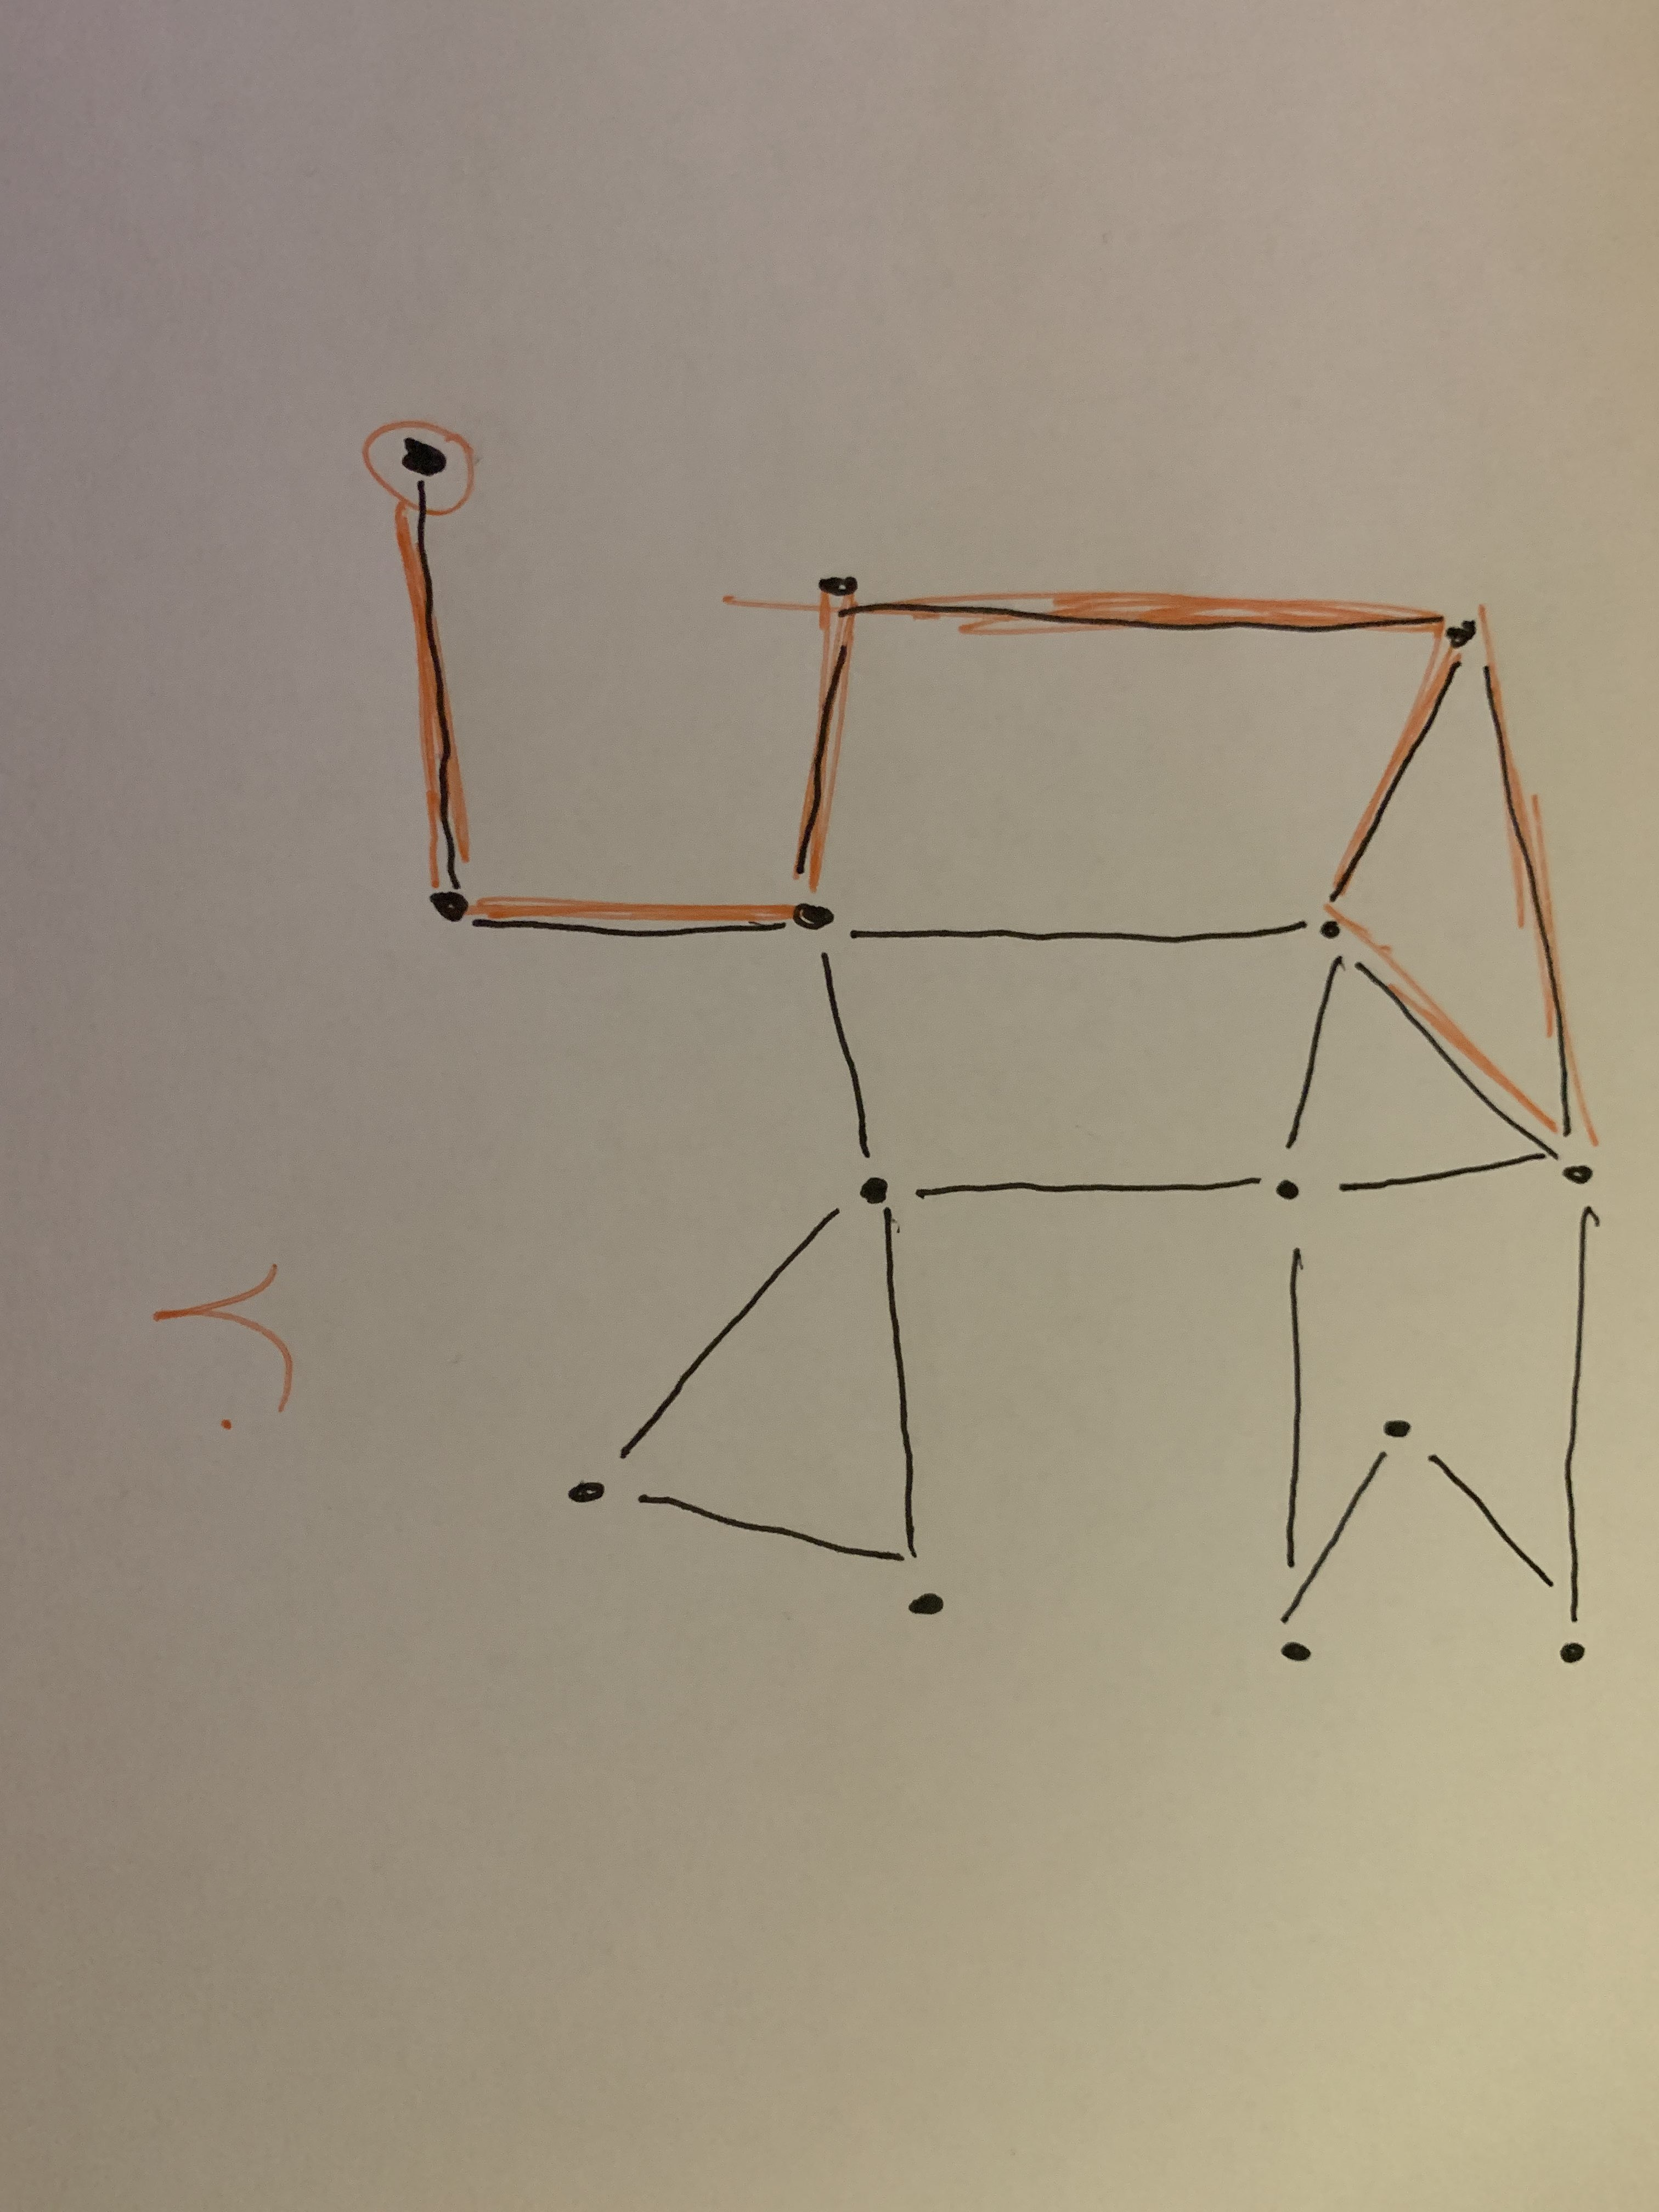
\includegraphics[width=0.25\textwidth]{IMG_4125.jpg}
            \caption{Solution for Problem 3 Part B}
        \end{figure}
        \item [(c)] Once the path $\gamma$ leaves the original vertex, it will be of odd degree, which would then mean for all other vertices, they will have an in and an associated out edge that the path can travel along to complete a path. However, for that odd edge of $v$ it is only an in and has no associated out edge.
        \item [(d)] See Figure 2 Below
        \begin{figure}
            \centering
            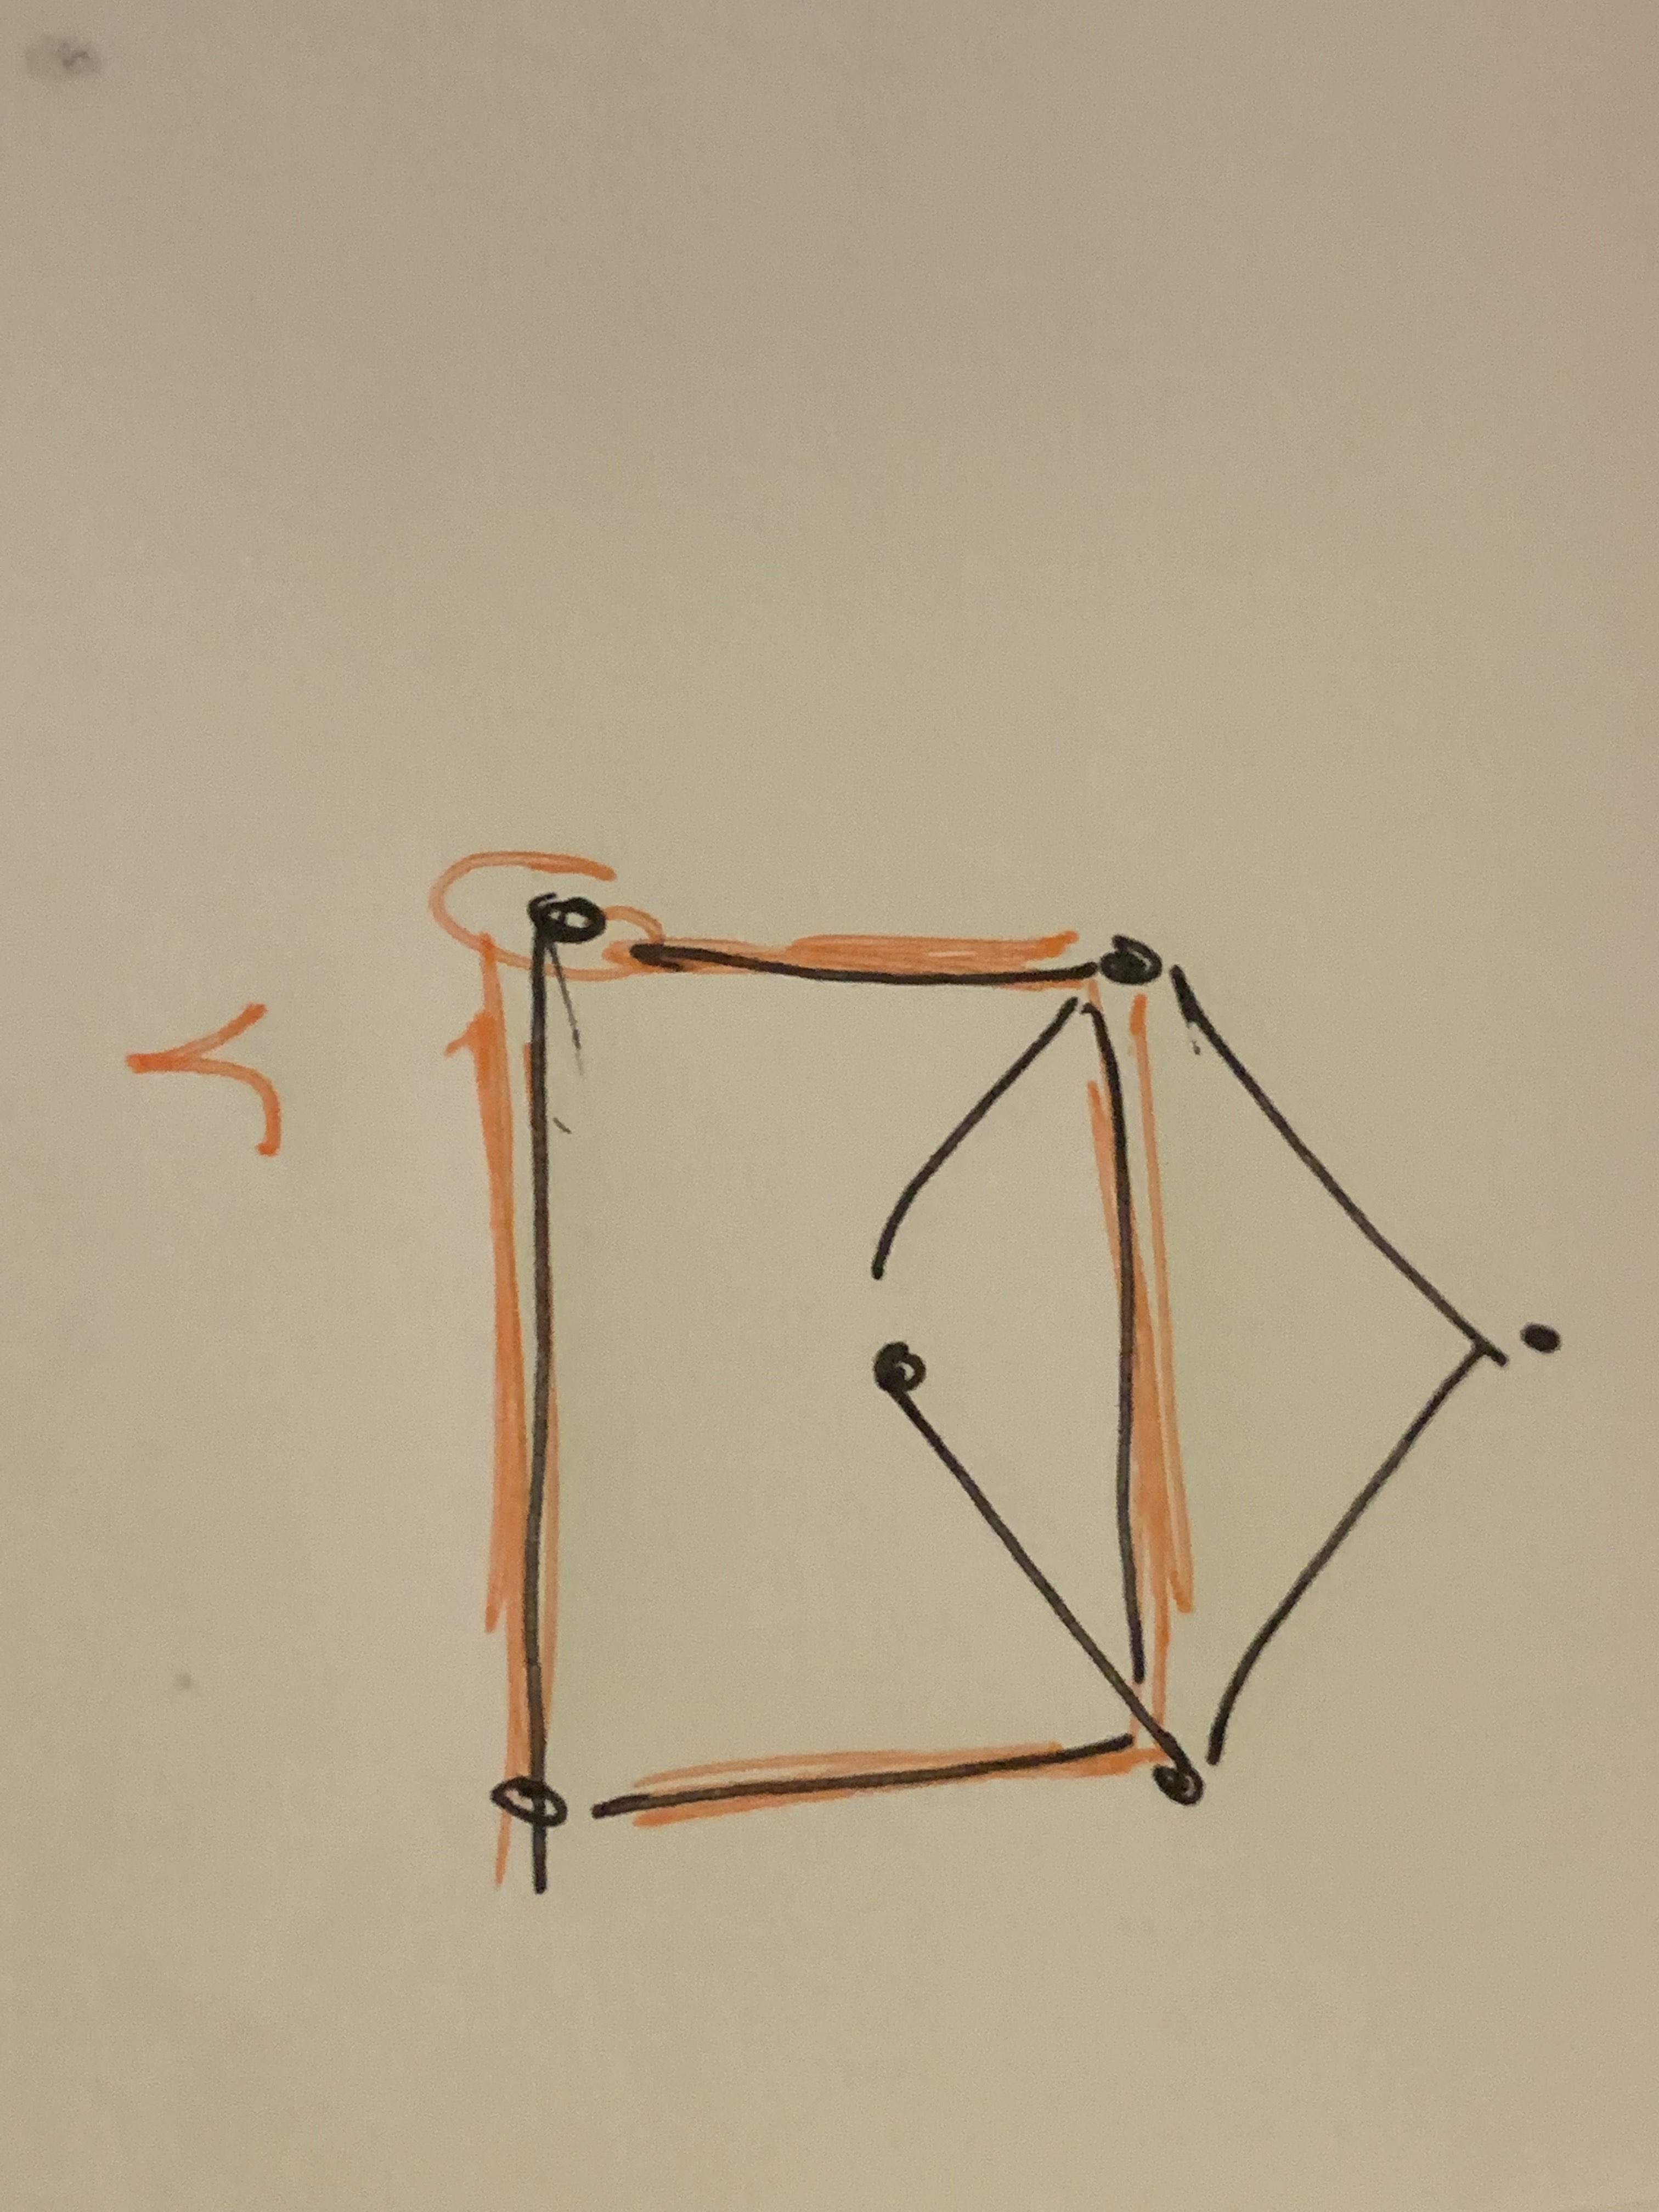
\includegraphics[width=0.25\textwidth]{IMG_4126.jpg}
            \caption{Solution for Problem 3 Part D}
        \end{figure}
        \item [(e)] All the edges that are removed by removing $\gamma$ will either be both pairs of an in and out from an even vertex and will remove both odd vertices if they were present in the graph $G$. Thus, the remaining graphs, while they might not been connected, will only have vertices of even degree.
        \item [(f)] We could remake $\gamma$ by instead of purely randomly picking edges to follow, we could prioritize edges that lead away from the known endpoint because we know that the paths, by above, will end in desired locations regardless.
        \item [(g)] For both graphs with either 2 odd vertices or no odd vertices will have an eulerian path because we can always construct a $\gamma$ that will use all edges and will end in known locations.
    \end{enumerate}
\clearpage

\begin{problem}
Let $d(x, y) := |x - y|$ be the usual distance on $\R$, and $d'$ be the distance by: $d'(x, y) := \min\{1, d(x, y)\}.$ Show that $d'$ is a distance and $d' \underset{top}{\sim} d$ while the two distances are not equivalent.
\end{problem}
\begin{claim}
$d'$ is a distance.
\end{claim}
\begin{proof}
    Let $x, y\in \R$, we know by definition that $d(x, y) \geq 0$ for all $x, y$;implying that $\min(1, d(x, y)) \geq 0$. Similarly, we know that for any $x, y\in \R$ that $\d(x, y) = d(y, x)$ by definition, again, implying that $d'(x, y) = \min(1, d(x, y)) = \min(1, d(y, x)) = d'(y, x) \Rightarrow d'(x, y) = d'(y, x)$. Lastly, we know that $d(x, y) \leq d(x, z) + d(z, y)$ for all $x, y, z \in \R$ by definition. Then we have three cases, where both of these distances are less than one, one of them is greater then or equal to one without loss of generality, or both of them are greater than or equal to one. In the first case then $\min(1, d(x, y)) \leq \min(1, d(x, z)) + \min(1, d(y, z)) = d(x, z) + d(y, z)$. Similarly, if one of them is greater than or equal to one, then $d'(x, y) = \min(1, d(x, y)) \leq \min(1, d(x, z)) + \min(1, d(y, z)) = 1 + d(x, z)$. And lastly, we know that $d'(x, y) \leq \min(1, d(x, z)) + \min(1, d(y, z)) = 1 + 1$ which we would then know $d'(1, d(x, y)) < 2$. Therefore, all the conditions are satisfied that $d'$ is a distance.
\end{proof}
It is simple to see that these distances are not always equal as the usual distance on $\R$ is not bounded by $1$. However now we want to show that $d' \underset{top}{\sim} d$:
\begin{proof}
    We have two cases we need to consider for this problem, if for $x, y\in \R$ if $d(x, y) < 1$ and $d(x, y) \geq 1$. We will first consider if $d(x, y) < 1$, then we know that $d'(x, y) = \min(1, d(x, y)) = d(x, y)$. Let $\alpha = 1$ and $\beta = 2$, then $1 * d(x, y) = d'(x, y) = \min(1, d(x, y)) < 2*d(x, y)$ which satisfies the condition. Now we consider the alternate case where $d(x, y) \geq 1$, then $d'(x, y) = 1$ so we set $\alpha = \frac{1}{d(x, y)}, \beta = 1$ we then know that $\frac{1}{d(x, y)}d(x,y) = d'(x, y) \leq d(x,y)$. This implies that $d_1 \sim d_2$ and since we know that the y are equivalent, then we know that they are equivalent topologically, hence $d \underset{top}{\sim} d'.$
\end{proof}
\clearpage

\begin{problem}
    Find all topologies on the set $\{a, b, c\}.$ Which are homeomorphic?
\end{problem}
We will define the set $X = \{a, b, c\}$. Then we have the trivial topology $\tau_1 = \{\emptyset, X\}$, then we have the simple insertions of singletons or doubletons to this topology $\tau_{2-7} = \{\emptyset, \{a\}, X\}, \{\emptyset, \{b\}, X\},$ $\{\emptyset, \{c\}, X\}, \{\emptyset, \{a, b\}, X\}, \{\emptyset, \{a, c\}, X\}, \{\emptyset, \{b, c\}, X\}$. Then we have the insertion of a singleton and its superset to get $\tau_{8 - 13} = \{\emptyset, \{a\}, \{a, b\}, X\}, \{\emptyset, \{a\}, \{a, c\}, X\}, \{\emptyset, \{b\}, \{a, b\}, X\},$\\ $\{\emptyset, \{b\}, \{b, c\}, X\}, \{\emptyset, \{c\}, \{a, c\}, X\}, \{\emptyset, \{c\}, \{b, c\}, X\}$. Then we have with each singleton and its compliment $\tau_{14-16} = \{\emptyset, \{a\}, \{b, c\}, X\}, \{\emptyset, \{b\}, \{a, c\}, X\}, \{\emptyset, \{c\}, \{a, b\}, X\}$. Then we have the topologies with a singleton and all supersets $\tau_{17 - 19} = \{\emptyset, \{a\}, \{a, b\}, \{a, c\}, X\},$\\ $\{\emptyset, \{b\}, \{a, b\}, \{b, c\}, X\}, \{\emptyset, \{c\}, \{a, c\}, \{b, c\}, X\}$. Then we insert a singleton and both corresponding supersets $\tau_{20 - 22} = \{\emptyset, \{a\}, \{b\}, \{a, b\}, X\}, \{\emptyset, \{a\}, \{c\}, \{a, c\}, X\}, \{\emptyset, \{b\}, \{c\}, \{b, c\}, X\}$. Then insert two singletons and two doubletons where the union of the two doubletons is one of the singletons $\tau_{23 - 28} = \{\emptyset, \{a\}, \{b\}, \{a, b\}, \{a, c\}, X\}, \{\emptyset, \{a\}, \{b\}, \{a, b\}, \{b, c\}, X\},$\\ $\{\emptyset, \{a\}, \{c\}, \{a, b\}, \{a, c\}, X\}, \{\emptyset, \{a\}, \{c\}, \{b, c\}, \{a, c\}, X\}, \{\emptyset, \{b\}, \{c\}, \{a, b\}, \{b, c\}, X\},$\\ $\{\emptyset, \{b\}, \{c\}, \{b, c\}, \{a, c\}, X\}$. Then lastly we have all permutations of $X$ for $\tau_{29} = P(X)$. This is for a total of $29$ topologies. Out of these topologies $\tau = \{\emptyset, X\}, \{\emptyset, \{a\}, \{b\}, \{c\}, \{a, b\}, \{a, c\}, \{b, c\}, X\},$\\ $\{\emptyset, \{c\}, X\}, \{\emptyset, \{a, b\}, X\}, \{\emptyset, \{c\}, \{a, b\}, X\}, \{\emptyset, \{c\}, \{b, c\}, X\}, \{\emptyset, \{a\}, \{b\}, \{a, b\}, X\},$\\$\{\emptyset, \{c\}, \{a, c\}, \{b, c\}, X\}, \{\emptyset, \{b\}, \{c\}, \{a, b\}, \{b, c\}, X\}$ are non-homeomorphic topologies on $X$ and the rest are homeomorphic.

\end{document}
